% !TeX spellcheck = fr-FR

\documentclass[intlimits, 10pt]{beamer}
\usetheme{Hannover}
\usecolortheme{crane}


%%% Pretty pretty
\setbeamercolor{alerted text}{fg=violet!80!black}
\setbeamercolor{background canvas}{bg=white}
\setbeamercolor{title}{fg=violet!80!black, bg=yellow!80!white}
\setbeamercolor{titlelike}{fg=violet, bg=yellow!80!white}
\setbeamercolor{sidebar}{bg=yellow!60!white}
\setbeamercolor{structure}{fg=violet!80!black}
\setbeamercolor{normal text}{fg=black}
\setbeamercolor{subsection in sidebar}{fg=violet!80!black}
\setbeamercolor{subsection in sidebar shaded}{fg=violet!40!gray}
\setbeamercolor{section in sidebar}{fg=violet!80!black}
\setbeamercolor{section in sidebar shaded}{fg=violet!40!gray}
\setbeamercolor{title in sidebar}{fg=violet!80!black}
\setbeamercolor{author in sidebar}{fg=violet!50!gray}
\setbeamercolor{block title}{fg=violet!80!black, bg=yellow!80!white}
\setbeamercolor{block body}{bg=yellow!15!white}

\addtobeamertemplate{navigation symbols}{}{%
	\usebeamerfont{footline}%
	\usebeamercolor[fg]{footline}%
	\hspace{1em}%
	\insertframenumber/\inserttotalframenumber
}

\usepackage{pfmathbeamer}
\usepackage{graphicx}
\usepackage{listings}
\lstset{
	backgroundcolor=\color{yellow!5!white},
	keywordstyle=\color{violet!80!black},
	numbers=left,
	frame=single,
	numberstyle=\tiny\color{violet!80!black},
	escapeinside={\%*}{*)},
	stringstyle=\color{black!10!yellow}
}


\hypersetup{pdfstartview=Fit}

\title[\textsc{Ernest'O'Clock}]{Projet de Systèmes Numériques}
\date{}
\author[\textsc{Fournier}, \textsc{Schabanel}, \textsc{Vivien}]{Paul \textsc{Fournier}, Juliette \textsc{Schabanel}, Samuel \textsc{Vivien}}

\DeclareMathOperator*{\argmin}{argmin}
\DeclareMathOperator*{\argmax}{argmax}
\newcommand{\bmm}[1]{\texorpdfstring{$\bm{#1}$}{#1}}

\AtBeginPart{\frame{\partpage}}
\AtBeginSection{\frame{\sectionpage}}
\AtBeginSubsection{\frame{\subsectionpage}}

\begin{document}
	\selectlanguage{french}
	
	\maketitle	
	
	\begin{frame}
		\tableofcontents
	\end{frame}
	
	\section{Microprocesseur}
	
	\begin{frame}{Caractéristiques}
		\begin{block}{Grandes idées}
			\begin{itemize}
				\item Peu d'instructions (pas de multiplication notamment)
				\item 32 registres de 32 bits
				\item Les mêmes drapeaux qu'en x86-64
				\item Code dans la ROM, mémoire dans la RAM
			\end{itemize}
		\end{block}
	\end{frame}
	
	\begin{frame}{Code machine}
		\begin{block}{Format des instructions}
			\begin{itemize}	
				\item 7 bits de code machine
				\item 1 bit d'écriture
				\item 16 bits de valeur d'entrée
				\item 2 bits de type de valeur d'entrée
				\item 5 bits de valeur de sortie
				\item 1 bit de valeur de sortie
			\end{itemize}
		\end{block}
	\end{frame}
	
	\begin{frame}[fragile, shrink]{Initialisation de l'horloge}
		\begin{lstlisting}[language={[x86masm]Assembler},morekeywords={lsr}, caption="Division euclidienne"]
			mov %r26 $86400
			mov %r25 %r26
			jmp "ew1"
			bw1:
			lsl %r25 $1
			ew1:
			cmp %r28 %r25
			jb "bw1"
			mov %r27 $0
			bw2:
			lsl %r27 $1
			cmp %r28 %r25
			ja "ew2"
			add %r27 $1
			sub %r28 %r25
			ew2:
			lsr %r25 $1
			cmp %r25 %r26
			jge "bw2"
		\end{lstlisting}
	\end{frame}
	
	\section{Compilation \texttt{.net} $\rightarrow$ \texttt{.c}}
	
	\begin{frame}{Compilation}
			\begin{table}
				\begin{tabular}{|c|c|}
				\hline
				Opérations sur les fils & Opérations sur les tableaux \\
				\hline
				Constante (\texttt{true} ou \texttt{false})& Constante ($0$ ou $1$)  \\
				\hline
				\texttt{not a}& \texttt{!a}  (nb: plus rapide qu'un \texttt{xor})\\
				\hline
				\texttt{and} & \texttt{\&}  \\
				\hline
				\texttt{or}& \texttt{|} \\
				\hline
				\texttt{xor}& \texttt{\^} \\
				\hline
				\texttt{a nand b }& \texttt{!(a \& b)} \\
				\hline
				\texttt{mux s b a}& \texttt{s?a:b} \\
				\hline
				\texttt{reg}&Assignation\\
				\hline
			\end{tabular}
			\caption{Traduction \texttt{.net} $\rightarrow$ \texttt{.c}}
		\end{table}
	\end{frame}
	
	\section{Interface homme machine}
	
	\begin{frame}{Format de l'affichage}
		\begin{figure}
			\centering
			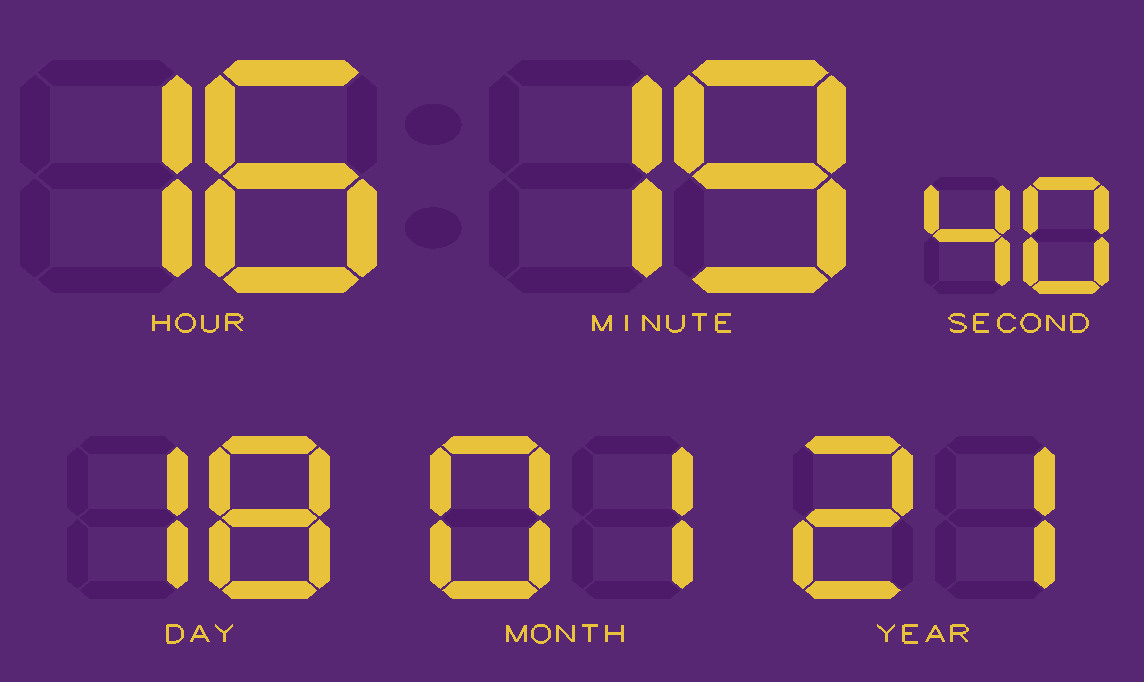
\includegraphics[width=0.7\linewidth]{../Rapport/2021-01-18_16-19}
			\caption{Démonstration statique de l'horloge}
			\label{fig:2021-01-1816-19}
		\end{figure}
		
	\end{frame}
	
	\begin{frame}{Memory-Mapped-Input-Output}
		\begin{table}
			\begin{tabular}{|c|c|c|c|c|c|}
				\hline
				$0-6$ & $7-13$ & $14-20$ & $21-27$ & $30$ & $31$ \\ 
				\hline
				Sec. 1 & Sec. 10 & Min. 1 & Min. 10 & Affichage? & Parité \\
				\hline
				\hline
				$33-39$ &$41-47$&$49-55$ &$57-63$ && \\
				\hline
				Heure 1 & Heure 10 & Jour 1 & Jour 10 &&\\
				\hline
				\hline
				$65-71$ & $73-79$ & $81-87$ & $89-95$ &&\\
				\hline
				Mois 1 & Mois 10 & Année 1 & Année 10 &&\\
				\hline
				\hline
				$128-159$ &&&&&\\
				\hline
				Init &&&&& \\
				\hline
			\end{tabular}
			\caption{Description de l'interface mémoire I/O}
		\end{table}
	\end{frame}
	
	\begin{frame}{Format MMIO}
		
		\begin{figure}
			\centering
			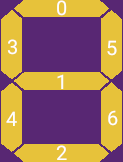
\includegraphics[width=0.3\linewidth]{../Rapport/segments}
			
			\begin{tabular}{|c|c|c|c|c|c|c|c|}
				\hline
				$b_0$& $b_1$  & $b_2$ & $b_3$ & $b_4$ & $b_5$ & $b_6$ & $b_7$ \\
				\hline
			\end{tabular}
			\caption{Représentation binaire de la sortie}
			\label{fig:segments}
		\end{figure}
		
		

	\end{frame}
	
\end{document}
